\documentclass[10pt,a4paper]{article}
\usepackage[T1]{fontenc}
\usepackage[spanish,es-noshorthands]{babel}
\usepackage{lmodern}
\usepackage[margin=2cm]{geometry}
\usepackage{graphicx}
\usepackage{booktabs,tabularx}
\usepackage{csquotes}
\usepackage[backend=biber,style=ieee,sorting=none,maxnames=3]{biblatex}
\usepackage{xurl}
\usepackage[hidelinks]{hyperref}
\addbibresource{referencias.bib}

\setlength{\parindent}{0pt}
\setlength{\parskip}{2pt}
\setlength{\emergencystretch}{1em}

\begin{document}

{\large Universidad Técnica Estatal de Quevedo}\par
{\small Aplicaciones Distribuidas · ISR-701 · GA-SUM-02 / EXP-1}\par
\vspace{.4em}
{\LARGE\bfseries Notas de la exposición}\par
{\large Mensajería Publish/Subscribe}\par

\section{Guion por integrante}

La presentación dura hasta 12 minutos. Cada integrante dispone de unos
3 minutos, incluida su demostración si corresponde. Al final se reservan
3 minutos para las preguntas.

% Cada fragmento incluye su propio encabezado con \subsection.
\subsection{Mario Zambrano · PUB/SUB aplicado al SGRA}

\paragraph{Arquitectura y problema identificado.}
El SGRA permite gestionar solicitudes de refuerzo académico
mediante Angular, Spring Boot y PostgreSQL. Actualmente, el
backend registra las solicitudes y gestiona notificaciones
por correo. Como propuesta de mejora, se plantea distribuir
eventos a componentes independientes, como notificaciones,
auditoría e indicadores \cite{sgra_backend}.

\paragraph{Fundamentos de Publish/Subscribe.}
PUB/SUB utiliza publicadores, un intermediario de mensajería
y suscriptores. El publicador no necesita conocer directamente
a cada receptor. Esto facilita el desacoplamiento y permite
procesar actividades complementarias de manera asíncrona
\cite{lazidis2022}.

\paragraph{Demostración y aplicación al SGRA.}
Primero se demuestra PUB/SUB con Mosquitto: un publicador
envía el evento \texttt{SolicitudTutoriaCreada} y dos
suscriptores reciben el mismo mensaje.

Posteriormente, se presenta la integración experimental
realizada en Java. Se incorporó Eclipse Paho al backend y
se ejecutaron pruebas de publicación, recepción, caída del
broker, recuperación y eventos duplicados.

Además, tres pruebas automatizadas con Mockito verificaron
el comportamiento del servicio ante registros exitosos,
fallos del registro y errores MQTT. Una prueba adicional
comprobó la publicación desde el servicio del SGRA hacia
Mosquitto y la recepción por dos suscriptores.

\paragraph{Resultados y limitaciones.}
Las pruebas confirmaron la distribución de eventos y
permitieron observar que una caída del broker impide nuevas
publicaciones mientras permanezca desconectado.

También se comprobó que dos publicaciones con el mismo
identificador lógico llegan a los suscriptores. Por ello,
una implementación completa necesitaría controlar duplicados
y recuperar publicaciones fallidas.

La persistencia se simuló mediante Mockito: no se ejecutó
una transacción real en PostgreSQL. Como mejora futura se
propone evaluar Transactional Outbox y consumidores
idempotentes para reforzar la consistencia y confiabilidad
\cite{microsoft2026}.


% Incorporar desde el documento grupal con % Incorporar desde el documento grupal con % Incorporar desde el documento grupal con \input{notas/carlos.tex}
% si el archivo principal está en la raíz. Las citas usan referencias.bib.

\subsection{Carlos Manotoa · MQTT aplicado a CLAB}

\paragraph{Arquitectura y comunicación.}
CLAB gestiona los laboratorios informáticos de la UTEQ. Cuando el
administrador marca una falla como resuelta, Angular envía una petición REST a
Spring Boot y espera su respuesta. El backend actualiza el reporte en
PostgreSQL, guarda el seguimiento y avisa al docente que reportó la falla.
Para el administrador, todo empieza con un botón. La aplicación se encarga del
acceso a la base de datos \cite[sección~3.2 y caso CU-04]{clab2026}.

\paragraph{Despliegue y CAP/PACELC.}
El diagrama muestra un servidor PostgreSQL. Si Spring Boot pierde la conexión
con ese servidor, no hay un mecanismo de conmutación automática documentado.
Para aplicar CAP y PACELC haría falta conocer la replicación, el comportamiento
ante particiones y cómo se resuelve el compromiso entre latencia y consistencia
en operación normal. El informe permite identificar la dependencia de la base
de datos, pero deja esos puntos abiertos \cite[figura~4]{clab2026}.

\paragraph{Fallo observado durante las pruebas.}
En una prueba con Postman, un bloqueo por evento institucional dejó sin aviso
a los docentes con reservas afectadas. El equipo corrigió una condición en
\texttt{BloqueoService} durante el mismo sprint. Para verificar el flujo
completo, comprobaría que se registre el bloqueo y se genere el aviso \cite[sección~6.5.2]{clab2026}.

\paragraph{Propuesta y demostración.}
Para la resolución de fallas, propongo guardar el evento pendiente en la misma
transacción que actualiza el reporte. Así, si Mosquitto está caído, un proceso
puede reintentar la publicación y el aviso se puede demorar sin deshacer la
resolución. En MQTTX publico \texttt{ReporteFallaResuelto} en
\texttt{clab/fallas/resuelta} y muestro el mismo mensaje en Notificaciones y
Auditoría. La demo comprueba la entrega a dos suscriptores conectados con QoS~1.
El broker distribuye por tópico. Con QoS~1, la confirmación es por tramo y
pueden llegar duplicados. Cada consumidor podría reconocerlos mediante
\texttt{eventoId} \cite{mqtt2019}.

% si el archivo principal está en la raíz. Las citas usan referencias.bib.

\subsection{Carlos Manotoa · MQTT aplicado a CLAB}

\paragraph{Arquitectura y comunicación.}
CLAB gestiona los laboratorios informáticos de la UTEQ. Cuando el
administrador marca una falla como resuelta, Angular envía una petición REST a
Spring Boot y espera su respuesta. El backend actualiza el reporte en
PostgreSQL, guarda el seguimiento y avisa al docente que reportó la falla.
Para el administrador, todo empieza con un botón. La aplicación se encarga del
acceso a la base de datos \cite[sección~3.2 y caso CU-04]{clab2026}.

\paragraph{Despliegue y CAP/PACELC.}
El diagrama muestra un servidor PostgreSQL. Si Spring Boot pierde la conexión
con ese servidor, no hay un mecanismo de conmutación automática documentado.
Para aplicar CAP y PACELC haría falta conocer la replicación, el comportamiento
ante particiones y cómo se resuelve el compromiso entre latencia y consistencia
en operación normal. El informe permite identificar la dependencia de la base
de datos, pero deja esos puntos abiertos \cite[figura~4]{clab2026}.

\paragraph{Fallo observado durante las pruebas.}
En una prueba con Postman, un bloqueo por evento institucional dejó sin aviso
a los docentes con reservas afectadas. El equipo corrigió una condición en
\texttt{BloqueoService} durante el mismo sprint. Para verificar el flujo
completo, comprobaría que se registre el bloqueo y se genere el aviso \cite[sección~6.5.2]{clab2026}.

\paragraph{Propuesta y demostración.}
Para la resolución de fallas, propongo guardar el evento pendiente en la misma
transacción que actualiza el reporte. Así, si Mosquitto está caído, un proceso
puede reintentar la publicación y el aviso se puede demorar sin deshacer la
resolución. En MQTTX publico \texttt{ReporteFallaResuelto} en
\texttt{clab/fallas/resuelta} y muestro el mismo mensaje en Notificaciones y
Auditoría. La demo comprueba la entrega a dos suscriptores conectados con QoS~1.
El broker distribuye por tópico. Con QoS~1, la confirmación es por tramo y
pueden llegar duplicados. Cada consumidor podría reconocerlos mediante
\texttt{eventoId} \cite{mqtt2019}.

% si el archivo principal está en la raíz. Las citas usan referencias.bib.

\subsection{Carlos Manotoa · MQTT aplicado a CLAB}

\paragraph{Arquitectura y comunicación.}
CLAB gestiona los laboratorios informáticos de la UTEQ. Cuando el
administrador marca una falla como resuelta, Angular envía una petición REST a
Spring Boot y espera su respuesta. El backend actualiza el reporte en
PostgreSQL, guarda el seguimiento y avisa al docente que reportó la falla.
Para el administrador, todo empieza con un botón. La aplicación se encarga del
acceso a la base de datos \cite[sección~3.2 y caso CU-04]{clab2026}.

\paragraph{Despliegue y CAP/PACELC.}
El diagrama muestra un servidor PostgreSQL. Si Spring Boot pierde la conexión
con ese servidor, no hay un mecanismo de conmutación automática documentado.
Para aplicar CAP y PACELC haría falta conocer la replicación, el comportamiento
ante particiones y cómo se resuelve el compromiso entre latencia y consistencia
en operación normal. El informe permite identificar la dependencia de la base
de datos, pero deja esos puntos abiertos \cite[figura~4]{clab2026}.

\paragraph{Fallo observado durante las pruebas.}
En una prueba con Postman, un bloqueo por evento institucional dejó sin aviso
a los docentes con reservas afectadas. El equipo corrigió una condición en
\texttt{BloqueoService} durante el mismo sprint. Para verificar el flujo
completo, comprobaría que se registre el bloqueo y se genere el aviso \cite[sección~6.5.2]{clab2026}.

\paragraph{Propuesta y demostración.}
Para la resolución de fallas, propongo guardar el evento pendiente en la misma
transacción que actualiza el reporte. Así, si Mosquitto está caído, un proceso
puede reintentar la publicación y el aviso se puede demorar sin deshacer la
resolución. En MQTTX publico \texttt{ReporteFallaResuelto} en
\texttt{clab/fallas/resuelta} y muestro el mismo mensaje en Notificaciones y
Auditoría. La demo comprueba la entrega a dos suscriptores conectados con QoS~1.
El broker distribuye por tópico. Con QoS~1, la confirmación es por tramo y
pueden llegar duplicados. Cada consumidor podría reconocerlos mediante
\texttt{eventoId} \cite{mqtt2019}.


\subsection{Nixon Piguave · JMS aplicado al RTV}
\noindent\textbf{Expositor:} Piguave Montaño Nixon Antonio. \textbf{Duración prevista:} 3 minutos, incluida la demostración.

\paragraph{Arquitectura JMS: 0:00--0:45.}
JMS, actualmente Jakarta Messaging, es una API de mensajería para Java. En nuestra práctica utilizamos Apache Artemis como proveedor: implementa las interfaces y administra la entrega.

El diagrama muestra un productor, un tópico y dos suscripciones independientes: auditoría e indicadores. En una cola, los consumidores compiten por los mensajes; en un tópico, cada suscripción puede recibir el evento. Por eso elegimos un tópico para que ambas funciones conozcan el inicio de una inspección. JMS define la API, no un protocolo de red único.\cite{jakarta2022}

\paragraph{Práctica: 0:45--2:00.}
La demostración utiliza datos ficticios y se ejecuta separada del RTV. La terminal A representa auditoría y la B, indicadores. Ambas están esperando en el tópico \texttt{rtv.inspecciones.iniciada}. Desde C publicaré \texttt{InspeccionIniciada} para el turno ficticio 42.

\noindent\textit{Acción: mostrar A y B, ejecutar en C y enseñar las dos recepciones. Reservar unos 20 segundos para cambiar de ventanas y esperar la salida.}
\begin{quote}\small\ttfamily
docker compose run --rm cliente publicar 42 evt-rtv-001
\end{quote}

El productor y ambos receptores muestran el mismo cuerpo y \texttt{JMSMessageID}. La ejecución demuestra difusión a dos suscripciones activas, no una inspección guardada en el sistema real. Las suscripciones son no durables: si cerramos sus consumidores, no conservarán los mensajes publicados durante su ausencia.

\paragraph{Aplicación propuesta: 2:00--3:00.}
En el RTV, Inspecciones pide autorización a Turnos y Pagos mediante REST antes de registrar el inicio. Proponemos publicar el evento después de guardarlo. Auditoría e indicadores podrían reaccionar sin llamadas directas desde Inspecciones a cada receptor.

Las líneas discontinuas representan esa propuesta. Debemos resolver qué ocurre si se guarda la inspección y falla la publicación, y cómo evitar efectos repetidos ante duplicados. En una futura integración con Spring podríamos usar \texttt{JmsTemplate} para publicar y \texttt{@JmsListener} para recibir.\cite{springjms}

Artemis sirvió para demostrar el mecanismo. Para elegir un proveedor en el proyecto, faltaría medir latencia y capacidad con nuestra carga; los resultados de otros estudios no son mediciones del RTV.\cite{maharjan2023} La autorización seguirá correspondiendo a Turnos y Pagos.


% Incorporar desde el documento grupal con % Incorporar desde el documento grupal con % Incorporar desde el documento grupal con \input{notas/john.tex}.
% Las citas usan referencias.bib.

\subsection{John Silva · AMQP aplicado al SSDC}

\paragraph{Arquitectura (0:00--0:35).}
En el SSDC, al aprobar una prepostulación, el mismo backend crea el usuario, envía las credenciales con una tarea \texttt{@Async} y registra la notificación; no hay broker. En RabbitMQ el productor publica en un \emph{exchange} y los \emph{bindings} deciden a qué colas llega el mensaje \cite{rabbitmq_concepts}. Propongo publicar \texttt{PrepostulacionAprobada} en un exchange \texttt{topic} con tres colas: correo, notificaciones y auditoría. Es una propuesta; el SSDC actual no la implementa.

\paragraph{Práctica (0:35--1:40).}
Con datos ficticios y tres consumidores esperando, publico tres eventos: la aprobación llega a las tres colas, el rechazo a correo y auditoría, y el cierre solo a auditoría. Si un consumidor está caído, el mensaje espera en su cola y se entrega al volver.

\paragraph{Comparación y recomendación (1:40--2:35).}
MQTT es ligero y pensado para dispositivos con poco ancho de banda; JMS es una API de Java; AMQP es un protocolo independiente del lenguaje \cite{oasis2012}. Un estudio pequeño con Raspberry Pi concluyó que AMQP transmitió más rápido que MQTT \cite{gultunca2018}, pero no mide el SSDC. Recomiendo AMQP con colas durables, confirmación manual y cola de fallidos; el costo es operar un componente más y aceptar consistencia eventual y duplicados \cite{maharjan2023}.

\paragraph{Incidente (2:35--3:00).}
El 2 de junio de 2019, un mantenimiento en una ubicación de Google Cloud detuvo a la vez el plano de control de red en varios clústeres, con pérdida de capacidad en seis regiones \cite{googlecloud19009}. Lección: no aplicar un cambio de configuración a todos los nodos del broker a la vez.

\paragraph{Pregunta para otro equipo.}
Si el servicio guarda el dato y el broker cae antes de publicar el evento, ¿cómo evitan que el dato quede guardado sin que nadie se entere?
.
% Las citas usan referencias.bib.

\subsection{John Silva · AMQP aplicado al SSDC}

\paragraph{Arquitectura (0:00--0:35).}
En el SSDC, al aprobar una prepostulación, el mismo backend crea el usuario, envía las credenciales con una tarea \texttt{@Async} y registra la notificación; no hay broker. En RabbitMQ el productor publica en un \emph{exchange} y los \emph{bindings} deciden a qué colas llega el mensaje \cite{rabbitmq_concepts}. Propongo publicar \texttt{PrepostulacionAprobada} en un exchange \texttt{topic} con tres colas: correo, notificaciones y auditoría. Es una propuesta; el SSDC actual no la implementa.

\paragraph{Práctica (0:35--1:40).}
Con datos ficticios y tres consumidores esperando, publico tres eventos: la aprobación llega a las tres colas, el rechazo a correo y auditoría, y el cierre solo a auditoría. Si un consumidor está caído, el mensaje espera en su cola y se entrega al volver.

\paragraph{Comparación y recomendación (1:40--2:35).}
MQTT es ligero y pensado para dispositivos con poco ancho de banda; JMS es una API de Java; AMQP es un protocolo independiente del lenguaje \cite{oasis2012}. Un estudio pequeño con Raspberry Pi concluyó que AMQP transmitió más rápido que MQTT \cite{gultunca2018}, pero no mide el SSDC. Recomiendo AMQP con colas durables, confirmación manual y cola de fallidos; el costo es operar un componente más y aceptar consistencia eventual y duplicados \cite{maharjan2023}.

\paragraph{Incidente (2:35--3:00).}
El 2 de junio de 2019, un mantenimiento en una ubicación de Google Cloud detuvo a la vez el plano de control de red en varios clústeres, con pérdida de capacidad en seis regiones \cite{googlecloud19009}. Lección: no aplicar un cambio de configuración a todos los nodos del broker a la vez.

\paragraph{Pregunta para otro equipo.}
Si el servicio guarda el dato y el broker cae antes de publicar el evento, ¿cómo evitan que el dato quede guardado sin que nadie se entere?
.
% Las citas usan referencias.bib.

\subsection{John Silva · AMQP aplicado al SSDC}

\paragraph{Arquitectura (0:00--0:35).}
En el SSDC, al aprobar una prepostulación, el mismo backend crea el usuario, envía las credenciales con una tarea \texttt{@Async} y registra la notificación; no hay broker. En RabbitMQ el productor publica en un \emph{exchange} y los \emph{bindings} deciden a qué colas llega el mensaje \cite{rabbitmq_concepts}. Propongo publicar \texttt{PrepostulacionAprobada} en un exchange \texttt{topic} con tres colas: correo, notificaciones y auditoría. Es una propuesta; el SSDC actual no la implementa.

\paragraph{Práctica (0:35--1:40).}
Con datos ficticios y tres consumidores esperando, publico tres eventos: la aprobación llega a las tres colas, el rechazo a correo y auditoría, y el cierre solo a auditoría. Si un consumidor está caído, el mensaje espera en su cola y se entrega al volver.

\paragraph{Comparación y recomendación (1:40--2:35).}
MQTT es ligero y pensado para dispositivos con poco ancho de banda; JMS es una API de Java; AMQP es un protocolo independiente del lenguaje \cite{oasis2012}. Un estudio pequeño con Raspberry Pi concluyó que AMQP transmitió más rápido que MQTT \cite{gultunca2018}, pero no mide el SSDC. Recomiendo AMQP con colas durables, confirmación manual y cola de fallidos; el costo es operar un componente más y aceptar consistencia eventual y duplicados \cite{maharjan2023}.

\paragraph{Incidente (2:35--3:00).}
El 2 de junio de 2019, un mantenimiento en una ubicación de Google Cloud detuvo a la vez el plano de control de red en varios clústeres, con pérdida de capacidad en seis regiones \cite{googlecloud19009}. Lección: no aplicar un cambio de configuración a todos los nodos del broker a la vez.

\paragraph{Pregunta para otro equipo.}
Si el servicio guarda el dato y el broker cae antes de publicar el evento, ¿cómo evitan que el dato quede guardado sin que nadie se entere?




\section{Tabla de aportes}

\begin{tabularx}{\textwidth}{@{}p{.37\textwidth}X@{}}
  \toprule
  \textbf{Integrante} & \textbf{Aporte documentado} \\
  \midrule
  Zambrano Parraga Luis Mario &
  Fundamentos de PUB/SUB, arquitectura del SGRA y práctica local de difusión. \\
  Manotoa Alava Carlos Alexander &
  MQTT con CLAB, diagramas TikZ, demostración con Mosquitto y MQTTX,
  evidencias y guion. \\
  Piguave Montaño Nixon Antonio &
  JMS con RTV, diapositivas y práctica con Apache ActiveMQ Artemis. \\
  Silva Triviño John Jairo &
  Análisis del SSDC y práctica de mensajería con RabbitMQ. \\
  \bottomrule
\end{tabularx}

\section{Declaración de uso de inteligencia artificial}

\textbf{Carlos Manotoa.} Se utilizó Codex como apoyo para la búsqueda y el filtrado de información, para la transformación rápida de contenido entre formatos (de txt a tex o md) y como apoyo en la resolución de los problemas encontrados. No obstante, la redacción, la revisión final y la documentación fueron realizadas y revisadas por el estudiante.

\textbf{Mario Zambrano.} Se utilizó ChatGPT como apoyo para la preparación de la integración Java--MQTT, las pruebas automatizadas y la documentación técnica. Ejecuté las pruebas en su entorno local y contrasté los resultados con las salidas de Maven y Mosquitto.

\textbf{John Silva.} Usé Claude (Anthropic) como apoyo para analizar el código del SSDC, preparar borradores de las diapositivas, del guion, revisar que el documento compilara. Ejecuté la práctica en mi equipo y tomé las capturas, abrí y verifiqué las fuentes citadas, y revisé y ajusté el contenido antes de entregarlo.


\textbf{Nixon Piguave.} Se utilizó Codex como apoyo para organizar el aporte de JMS, consultar fuentes, documentar en latex y preparar borradores de código, configuración Docker, diagramas TikZ. Ejecuté manualmente la práctica y las capturas, y las bitacoras fueron hechos por mi mismo. 

\begingroup\footnotesize
\printbibliography[heading=bibnumbered]
\endgroup

\appendix
\section{Bosquejo inicial de arquitectura}

\IfFileExists{evidencias/Boceto_inicial_a_papel.jpg}{
    \begin{center}
        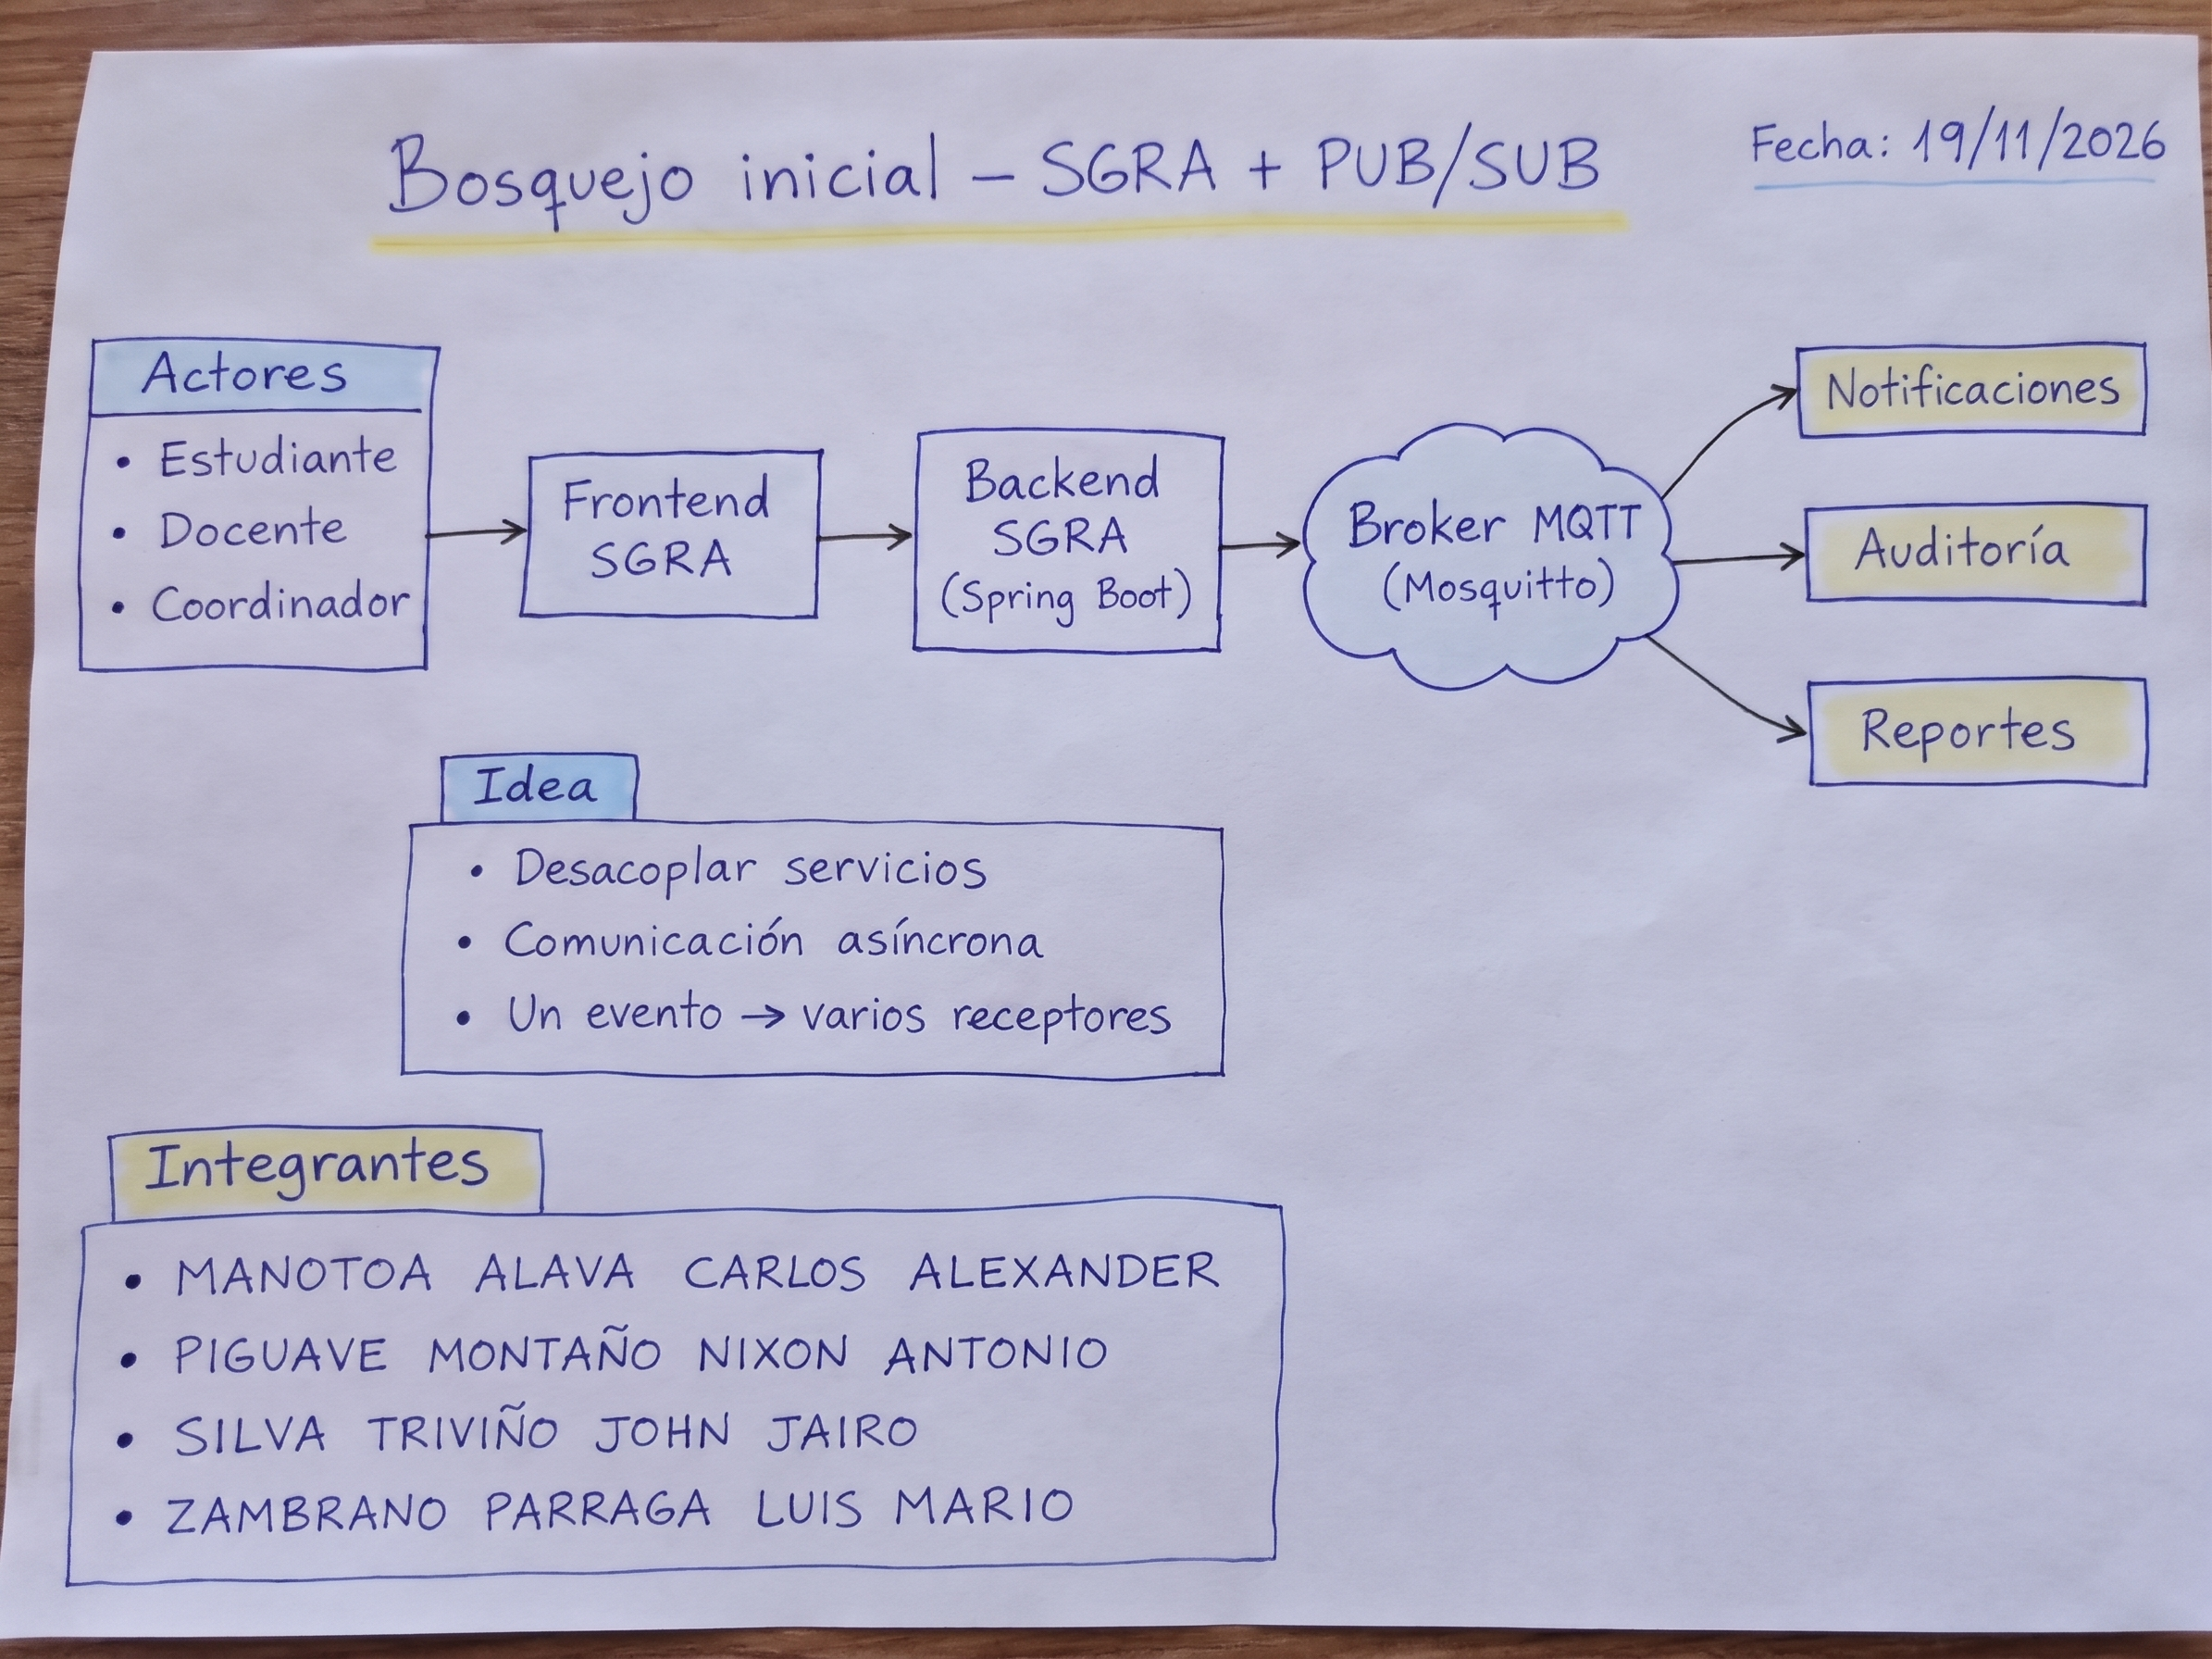
\includegraphics[
            width=\linewidth,
            height=.30\textheight,
            keepaspectratio
        ]{evidencias/Boceto_inicial_a_papel.jpg}
    \end{center}
}{
    \emph{Pendiente de incorporar el bosquejo.}
}

\end{document}
